\subsection{Factorizacion QR}
\textbf{Definicion:} Se dice que una matriz tiene \textbf{factorizacion QR} si puede ser expresada de la forma
\begin{center}
A = Q*R
\end{center}

El algoritmo para llevar a una matriz a su forma QR tiene costo $O(n^3).$ Tiene la misma ventaja que la factorizacion LU de permitir resolver un sistema de ecuaciones en orden $O(n^2)$, pero con la ventaja que \textbf{toda matriz tiene factorizacion QR}

\begin{center}
Ax = b

QR x = b

$Q^t$ Q R x = $Q^t$ b

R x = $Q^t$ b

con Rx un \textbf{sistema triangular superior}
\end{center}

Para poder calcular la matriz R se pueden aplicar los metodos de \textbf{Givens o Householder}

\subsubsection{Given}

Para eliminar el elemento en la posicion (i,j) aplicamos la siguiente matriz:

\begin{figure}[H] 
\begin{center}
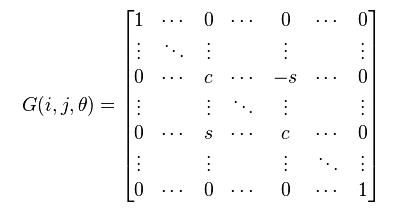
\includegraphics[width=0.5\textwidth]{img/givens.png} 
\caption{Matriz de Givens} 
\end{center}
\end{figure}

con c = cos($\theta$) y s = sen($\theta$). Luego aplicando G(i,j,$\theta$) * A queda en 0 el elemento (i,j). Entonces aplicamos sucesivamente este procedimiento para todos los elementos que queremos poner en 0 obteniendo asi nuestra matriz R. Luego $Q^t$ =  $\prod_{i = n}^1 G_i $

\subsubsection{Householder}

Con este metodo vamos e limando los 0 de abajo de la diagonal columna a columna.
Sea x = $col_i(A)$, y = ( $||x||_2$, 0 ,. . . 0) y sea $u$ = x - y. Definimos $H_i$ = I -  $ \frac{2uu^t}{u^tu} $.
Luego aplicando $H_i$ * A queda triangulada la columna i de A. Aplicamos este procedimiento iterativamente sobre $A^{(i)}$ hasta dejar triangulada la matriz. 
Quedando $Q^t$ =  $\prod_{i = n}^1 H_i $
